\subsection{The motivation for and structure of realistic LIV}
\label{ssec:LV}
%
%
The absence of a predictive theory of quantum gravity
with accompanying low-energy signals
remains an open problem. Early work in
string theory demonstrated that 
if additional tensor-valued fields $T^{\mu\nu\cdots}$
obtained a nonzero vacuum expectation value (vev)
this could lead to the spontaneous violation of 
Lorentz and CPT symmetry~\cite{Kostelecky:1988zi,Kostelecky:1991ak}. 
These vevs would generate additional interactions
in an effective fermion theory at low energies 
with schematic form~\cite{Kostelecky:1991ak}
%
\begin{equation}
\label{lowE}
\mathcal{L}_{\text{LV}} \sim 
\frac{\lambda}{M^{k}}\braket{T}\cdot
\bar{\psi}\Gamma(i\partial)^{k}\psi+ \text{h.c.},
\end{equation}
%
where $\lambda$ is a coupling constant, 
$M$ is the scale of new physics 
(perhaps, but not necessarily, the Planck scale), $k$ is a positive 
integer and $\braket{T} \equiv \braket{T^{\mu\nu\cdots}}$ 
represents tensor-valued vev contracted with the gamma-matrix
structure $\Gamma$ (with suppressed Lorentz indices) in 
the fermion bilinear product to its right, and h.c. stands
for Hermitian conjugation. 
The vev $\braket{T}$ breaks the four-dimensional Lorentz
invariance because it has Lorentz indices 
which ``point" in some direction. 
Experiments with sufficient sensitivity to measure the 
combination $\lambda \braket{T}/M^k$ could 
indirectly probe certain classes of string theories.
%This scenario contrasts with that of the SM Higgs mechanism, 
%where the associated vev $\sim \braket{\phi} = v \neq 0$ is simply a scalar.

Sustained interest in the possibility
of Lorentz violation as a realistic 
low-energy signal of Planck-scale
physics has come from other string-based approaches
\cite{Ellis:2008gg,Gliozzi:2011hj,Hashimoto:2012ig}, 
loop quantum gravity \cite{Gambini:2014kba,Rovelli:2010ed}, 
noncommutative field theories \cite{Carroll:2001ws,Carlson:2001sw,
Calmet:2004ii,Calmet:2004dn,Bailey:2018ifc}, 
high-energy electrodynamics and cosmic rays \cite{Carroll:1989vb, 
Coleman:1998ti}, and modified theories of gravity
\cite{Kostelecky:2020hbb,Kostelecky:2021xhb,
Kostelecky:2021tdf,deRham:2014zqa,Horava:2009uw,
Bluhm:2004ep,Bluhm:2007bd,Bluhm:2014oua}. Here we use
the adjective ``realistic" in the sense of those high-energy mechanisms/models
generating LIV that map onto low-energy effective field theories 
with desirable properties including energy-momentum conservation, 
locality, the SM gauge structure, etc., except 
(particle) Lorentz and CPT invariance. We work at the level of realistic
effective field theory and do not assume any particular 
high-energy mechanism inducing LIV.

LIV terms like~\eqref{lowE} have some unconventional properties
that are best understood by example.
Consider the following term:
\begin{equation}
\label{bterm}
\mathcal{L}_b = -b_\mu \bar \psi \gamma_5\gamma^\mu \psi.
\end{equation}
Here, the coefficient $b_\mu = (b_0,b_j)$ may be thought of as a vector vev.
Comparing $\mathcal{L}_b$ to the generic $\mathcal{L}_{\text{LV}}$ in 
Eq.~\eqref{lowE} shows that $b_\mu \leftrightarrow 
\lambda \braket{T}/M^0 =  \lambda \braket{T}$
and $\Gamma(i\partial)^0 \leftrightarrow \gamma_5\gamma^\mu$. 
In natural units, power counting indicates the 
mass dimension of the coefficient is $[b_\mu] = $\; GeV. As the Lorentz
index $\mu$ is contracted, $\mathcal{L}_b \rightarrow \mathcal{L}_b$ is invariant under Lorentz
transformations of the coordinate system, known as observer Lorentz transformations~\cite{ck97}.
If, in contrast, the \textit{physical system} $\psi$ is rotated, boosted, or some combination of both
while leaving the coordinates unaffected, 
then generically $\mathcal{L}_b \not\rightarrow \mathcal{L}_b$. 
This is known as a particle Lorentz transformation.
Under a particle transformation, $b_\mu \rightarrow b_\mu$, but
$\psi(x)$ transforms 
in general to a different field $\psi'(x)$ 
evaluated at the same spacetime point $x$. Thus, 
the full term ${\cal L}_b$ transforms to a distinct term
$\mathcal{L}'_b \neq \mathcal{L}_b$.
The reason $b_\mu$ is unaffected by particle transformations
is because it can be viewed as a 
background vector-valued field at 
every point in the vacuum, analogous
to the SM Higgs scalar background but including an orientation.
Terms like Eq.~\eqref{bterm} therefore only describe Lorentz-violating 
effects associated to the noninvariance under 
particle Lorentz transformations. 
To reiterate, ${\cal L}_b$ is invariant under observer transformations.
This is a desirable feature, because coordinate choices (i.e. changes
in the observer's perspective) 
are arbitrary---they should not affect the physics.
The ability to distinguish between particle and observer transformations
implies Lorentz invariance is violated. 

Equation~\eqref{bterm} also describes a 
CPT-violating effect because $\bar \psi \gamma_5\gamma^\mu \psi \rightarrow
-\bar\psi \gamma_5\gamma^\mu \psi$ under the operation of CPT and $b_\mu\rightarrow b_\mu$
because the CPT operation is necessarily a type of particle transformation. 
Thus, ${\cal L}_b \rightarrow -{\cal L}_b$ under a CPT transformation and is therefore CPT odd.

The equations of motion of a system follow from the Euler-Lagrange equations.
Performing particle transformations can change the
Lagrange density of terms like ${\cal L}_b$ in a nontrivial way. Thus, the system $\psi$ can experience
different equations of motion depending on its relative orientation to the background
field $b_\mu$. For example, one could perform a measurement where the laboratory apparatus
(containing the particle content associated to $\psi$) is initially upright. 
A second measurement could then be performed except with an
the apparatus in a horizontal position. By comparing the two measurements 
one could, in principle, infer the existence of $b_\mu$. This general idea will
be expounded upon when we discuss sidereal oscillations 
of event observables in the following subsections. 
%
%
\subsection{Standard-Model Extension (SME)}
\label{ssec:SME}
%
%
The Lagrange density ${\cal L}_b$ in Eq.~\eqref{bterm} is actually one
among many that appear in the model-independent 
effective field theory~\cite{Weinberg:2009bg} for Lorentz 
and CPT violation, known as the Standard-Model Extension (SME)
~\cite{ck96,ck98}. By construction, the SME provides a
model-independent parameterization
of all possible Lorentz-violating effects
constructed from SM and gravitational fields.
Each term in the SME can be thought of as
the product of a coefficient
for Lorentz violation
\footnote{For brevity 
we collectively refer to the 
coefficients for Lorentz (and possibly) CPT 
violation as ``SME coefficients". The SME coefficients
are sometimes called Wilson coefficients, given
they appear in an effective field theory. We refrain 
from using this latter terminology to avoid 
confusion with it usage in Lorentz-invariant effective
field theories.} 
of mass dimension $4-d$
with a Lorentz-violating field operator of dimension $d$.
For example, in ${\cal L}_b$ the coefficient for Lorentz violation is $b_\mu$
and the Lorentz-violating field operator is $-\bar\psi \gamma_5\gamma^\mu \psi$.
Because this field operator is mass dimension $d=3$, the coefficient for
Lorentz violation is of mass dimension $4-3=1$, as claimed.
CPT violation is also parametrized by the SME,
since for local and unitary quantum field theories,
when CPT invariance is violated, so too
is Lorentz invariance~\cite{ck97,owg}.
All SME terms violate Lorentz invariance, but the general pattern is
that those coefficients with odd numbers
of Lorentz indices also violate CPT invariance\footnote{This is true in the vast majority
of cases. There are two known exceptions,
but these cases involve SME coefficients which are irrelevant
for our study.}.

Our program will be based on the conservative approach of the SME. The SME
Lagrange density can be written as 
%
\begin{equation}
\label{SMEaction}
{\cal L}_{\text{SME}} = {\cal L}_{\text{SM}} + \delta {\cal L}_{\text{LV}},
\end{equation}
%
where ${\cal L}_{\text{SM}}$ is the SM Lagrange density 
and $\delta{\cal L}_{\text{LV}}$ represents all possible 
Lorentz-violating terms consistent with the SM field content and
$SU(3)\times SU(2)\times U(1)$ gauge structure. Experimental results
suggest it is reasonable to take $\delta{\cal L}_{\text{LV}}$ as
perturbations with respect to ${\cal L}_{\text{SM}}$. This is equivalent
to saying the coefficients for Lorentz violation are treated as perturbative
quantities with respect to the mass scales appearing in the process of interest. 

SME operators of mass dimension $d\leq 4$ 
are power-counting renormalizable and part of the \textit{minimal} SME.
There are a finite number parameters in the minimal SME. This is the theory
obtain by taking the SM and relaxed the conditions
of particle Lorentz and CPT invariance.
In contrast, operators with $d>4$ are power-counting nonrenormalizable and infinite
in number. They are part of the \textit{nonminimal} SME. Just as with 
Lorentz invariant nonrenormalizable theories like the Standard Model Effective
Field Theory (SMEFT), the nonminimal SME takes on a particular importance
in high-energy process like collider processes. Our program considers
both minimal and nonminimal SME effects. 

To summarize, the SME provides a rigorously justified
analysis framework for probing
generic Lorentz- and CPT violating effects
in experiments. This is evidenced by the hundreds 
of constraints placed using the SME over the past two decades~\cite{datatables}.
Despite the impressive progress, some
sectors of the SME, including the quark- and electroweak
sectors, remain largely unexplored.
In the proceeding sections, we describe recent progress
on this front and the role existing
ATLAS Drell-Yan measurements will play in expanding the 
search for Lorentz violation.
%
%
\subsection{Summary of SME studies involving quarks, gluons, and hadrons}
\label{ssec:prevstudies}
%
%
Briefly reviewing existing studies involving 
Lorentz-violating effects in quarks and gluons (partons) 
and hadrons puts our search into context.

Beginning at the lowest mass dimension $d = 3$, 
``$a$-type" effects $-a_\mu \bar\psi \gamma^\mu \psi$ 
have been constrained over a range of ten orders 
$\lesssim 10^{-12}$-$10^{-22}$\;GeV from 
$K, D, B_d$, and $B_s$ meson oscillations, and
from mapping quark-level coefficients to meson-level effective
coefficients using chiral perturbation theory ($\chi$PT)
~\cite{Kostelecky:1997mh, Kostelecky:1999bm, Kostelecky:2000ku, 
Isgur:2001yz, Nguyen:2001tg, Babusci:2013gda, Kostelecky:2001ff, 
Aubert:2007bp, Kostelecky:2010bk, Abazov:2015ana, 
Aaij:2016mos, Roberts:2017tmo, Schubert:2016xul,Altschul:2019beo}. 
Similar techniques have led to $d=5$ constraints 
on $K, D, B_d$, and $B_s$ meson 
effects~\cite{Edwards:2018lsn, Edwards:2019lfb}. 
The combination of $\chi$PT with 
astrophysical measurements have produced
various levels of sensitivity to 
$d=4$ ``$c$-type" effects $c_{\mu\nu}\bar\psi i\partial^\mu\gamma^\nu \psi$ 
on light quark ($u$, $d$) coefficients and 
``$k$-type" gluon effects 
$-\tfrac{1}{4}k^{\mu\nu\alpha\beta}G^{a}_{\mu\nu}G^{a}_{\alpha\beta}$, respectively
~\cite{Kamand:2016xhv,Kamand:2017bzl,Altschul:2019beo,
Noordmans:2016pkr,Noordmans:2017kji}. 
Similar constraints on light quarks 
have been placed considering 
the absence of photon decay 
and vacuum Cherenkov radiation 
\cite{Gagnon:2004xh, Altschul:2006uw, Kostelecky:2013rta, Schreck:2017isa}. 
Constraints on heavy quarks (the second and third generation)
are few in comparison and are typically
substantially weaker than those on light quarks. 
A few bounds have resulted from LEP 
data~\cite{Karpikov:2016qvq}, 
$t\bar t$ production at Fermilab 
and the LHC~\cite{Berger:2015yha,Abazov:2012iu,Carle:2019ouy},
radiative corrections to the photon propagator~\cite{Satunin:2017wmk}, 
and potentially stable top-flavored hadrons~\cite{Altschul:2020wkw}

%Colliders operate in the 
%$\sim 10^2$-$10^4$\;GeV range
%are situated between the typically $\sim$ eV-MeV range 
%of low-energy experiments
%involving atomic, mesonic and baryons systems 
%and that of the most energetic cosmic rays observed, which  
%exceed LHC energies by over 7 orders of magnitude. 
%Despite the substantial reduction in energy over
%cosmic-ray observations 
A number of leading constraints in the electron
and photon sectors have been placed with collider data. 
However, these constraints are limited to the
rotationally invariant combinations 
of the SME coefficients~\cite{Altschul:2009xh,Altschul:2010na,kl19}.
Most of the SME coefficients are not rotationally invariant.
Colliders have some advantages over other experiments
in constraining the larger set of rotation-violating subsets 
of SME coefficients. These advantages include
the large number of events collected semi-regularly
over long durations (many months to years). 
%and control over colliding beamlines. 
These features make collider experiments suitable for 
\textit{sidereal analyses}, which track the oscillation of
an observable as a function of the Earth's 
sidereal period $\sim$ 23 hrs 56 mins. 
This technique was utilized in Ref.~\cite{Abazov:2012iu}
to place the constraints on several components 
of the top-quark $c$- and $d$-type 
coefficients (see the following subsection).

Advances in theory and phenomenology (by
theory STA members of our program)
have enabled arbitrary-dimension $d$
quark-sector effects to be incorporated in
perturbative hadronic process, in particular
deep inelastic scattering and the Drell-Yan process 
~\cite{Kostelecky:2016pyx, Lunghi:2018uwj, Kostelecky:2019fse,lssv21}. 
We note that gauge-sector Lorentz violation (e.g. involving Lorentz-violating effects
in the $Z$ boson itself) have also
been considered in Refs.~\cite{Fu:2016fmf, Colladay:2017zen, Michel:2019tti}, 
though these considerations lie outside our current goals.

Focusing on the developments in
Refs.~\cite{Kostelecky:2016pyx, Lunghi:2018uwj, Kostelecky:2019fse,lssv21}, 
we show that ATLAS data of Drell-Yan 
events on the $Z$-boson pole result 
in first constraints on the chiral ``$d$-type" coefficients, 
which are particularly challenging to probe, 
and derive competitive constraints on
the $c$-type coefficients (introduced above). 
%
%
\subsection{Minimal quark-sector effects}
\label{ssec:canddtype}
%
%
Our primary interest is to investigate the leading
quark-sector effects\footnote{By ``leading" we mean those SME operators
of most relevance to the considered process of dilepton production. 
%For more information see Sec.~\ref{ssec:theorydetails}.
}.
They are given by three terms in the quark sector of the SME:
%
\begin{align}
\label{model1}
\mathcal{L} &= \tfrac{1}{2}i c_{Q_i}^{\mu\nu}\overline{Q}_i\gamma_\mu\overset{\text{\tiny$\leftrightarrow$}}{D}_\nu Q_i  
+ \tfrac{1}{2}i c_{U_i}^{\mu\nu}\overline{U}_i\gamma_\mu\overset{\text{\tiny$\leftrightarrow$}}{D}_\nu U_i 
 + \tfrac{1}{2}i c_{D_i}^{\mu\nu}\overline{D}_i\gamma_\mu\overset{\text{\tiny$\leftrightarrow$}}{D}_\nu D_i \;,
\end{align}
where $D_\nu$ is the conventional (SM) covariant derivative. 
The fields have the usual definitions
\begin{align}
Q_i = \begin{pmatrix} u_i \\ d_i \end{pmatrix}_L, \quad U_i = \left(u_i\right)_R, \quad D_i = \left(d_i\right)_R.
\end{align}
%
The index $i = 1, 2, 3$ denotes flavors $u_i = (u, c, t)$ and 
$d_i = (d, s, b)$ and the SME coefficients are given 
by $c_{Q_i}^{\mu\nu}$, $c_{U_i}^{\mu\nu}$, and $c_{D_i}^{\mu\nu}$. 
They may be taken as symmetric and traceless matrices, leaving
nine independent components per type $Q, U, D$. 
It is customary and useful to define the combinations
%
\begin{align}
\label{eq:quarkcoeffs}
c_{u_i}^{\mu\nu} &= (c_{Q_i}^{\mu\nu} + c_{U_i}^{\mu\nu})/2, \quad c_{d_i}^{\mu\nu} = (c_{Q_i}^{\mu\nu} + c_{D_i}^{\mu\nu})/2  \;, \nonumber\\
d_{u_i}^{\mu\nu} &= (c_{Q_i}^{\mu\nu} - c_{U_i}^{\mu\nu})/2, \quad d_{d_i}^{\mu\nu} = (c_{Q_i}^{\mu\nu} - c_{D_i}^{\mu\nu})/2  \;,
\end{align}
%
with the constraint $c_{u_i}^{\mu\nu} -c_{d_i}^{\mu\nu} 
= d_{d_i}^{\mu\nu} - d_{u_i}^{\mu\nu}$. As suggested by the subscripts, 
we refer to these latter coefficients as the $c$- and $d$-type coefficients. 
When expressing the Lagrange density~\eqref{model1} in terms of mass eigenstates, 
the $d$-type coefficients are contracted with a Lorentz-violating operator
$\bar\psi(i\partial_\mu)\gamma_5\gamma_\nu \psi$ and therefore are
associated with a chiral current. 
%
%
\subsection{LIV effects in the Drell-Yan process}
\label{ssec:LIVDY}
%
%
Direct probes of the $c$- and $d$-type coefficients 
are typically frustrated by QCD confinement. However, 
perturbative QCD factorization is known to be maintained
in the presence of these coefficients. Analytical
results for the scattering cross sections
are thus possible and are available for analysis. 
%
The $d$-type coefficients introduce additional
complications relative to the $c$-type coefficients.
In contrast to the $c$-type coefficients, the 
$d$-type coefficients modify the polarization properties of quarks.
It turns out this makes them significantly harder to probe. 
For example, the presence of virtual gluons inside
a hadron imply a given quark
does not have a well-defined spin.
For a spin-zero meson, the net spin from 
valence quarks must 
average to zero. This means that even if the 
$d$-type effects are present
they average to zero and are unobservable 
in spinless mesons like pions. 
%
It has also been emphasized~\cite{ls18} that 
unpolarized hadronic processes
mediated by a photon or gluon
are also insensitive to $d$-type
coefficients, due to the opposite-sign 
contributions in the scattering amplitudes.

The only known ways to probe the $d$-type coefficients
are with unpolarized beams exchanging a $W$ or $Z$ boson,
or though polarized beamlines. Since no currently operating
colliders fall into the latter category, this leaves
the LHC as the sole experiment 
for probing the $d$-type coefficients. 

%% One alternative is to consider polarized beamlines,
%% however no existing collider is 
%% relevant in this context. In contrast, 
%% for electroweak-mediated processes there
%% \textit{is} the possibility to probe the
%% effects of the $d$-type coefficients, 
%% due to the inequality of left- and right-handed
%% couplings to the $Z,W^{\pm}$~\cite{lssv21}. 
%% This method is the only known possibility to independently
%% and directly probe the $d$-type quark coefficients
%% with existing collider data. The Drell-Yan process
%% is a perfect candidate signal because 
%% data exists in the invariant mass region where
%% the $Z$-boson goes on shell, which is also where sensitivity
%% to the $d$-type coefficients are maximal.
%% In contrast, for a similar process like deep inelastic scattering,
%% the exchanged $Z$ relative to photon $t$-channel exchange is greatly 
%% suppressed. 
With regard to the
$c$-type coefficients, the bounds
we expect to obtain~\cite{ls18,klsv19}
will not be competitive with existing 
first-generation limits. However, we will also 
probe distinct linear coefficient combinations and
the second-generation ($s,c$). The latter
constraints will exceed the few existing ones by 
by a two or so orders of magnitude~\cite{Karpikov:2016qvq}.
As suggested, the $d$-type coefficients are the most 
motivated and uniquely suitable for study
using ATLAS data of the Drell-Yan process 
on the $Z$-boson pole.
%
%
\subsection{Dilepton distribution}
\label{ssec:DYxsec}
%
%
This section summarizes the cross section calculations relevant
for our analysis and described in Refs.~\cite{Kostelecky:2019fse,lssv21}.
%It is emphasized that 
%unpolarized DY process in the ultrarelativistic limit, through $\gamma/Z$ 
%interference and pure $Z$ exchange, provides a natural avenue for 
%accessing and constraining these coefficients. Note that effects 
%of Lorentz violation on the $Z$ boson have also been studied 
%in similar processes \cite{Fu:2016fmf, Colladay:2017zen, Michel:2019tti}, 
%however, these considerations are outside the scope of this work. 
%The leading-order cross section as a function of 
%the dilepton invariant mass is derived.  Coupled with data on $Z$-boson 
%production from the LHC, real and simulated constraints are 
%placed on the coefficients for Lorentz violation for $u, d, s,$ and $c$ quarks
%
%

The leading-order Drell-Yan dilepton distribution
$d\sigma/dQ^2$ including photon, 
photon-$Z$ interference, and pure $Z$ exchange including 
the effects from Eq.~\eqref{model1} is \footnote{Recalling the assumption that the LIV effects are small relative to the SM contributions, we work at 
first-order in the SME coefficients, disregarding 
the highly suppressed quadratic (and all higher-order) corrections.}\footnote{Note this is Eq. (3.14) in Ref.~\cite{lssv21}, except here
the prefactor for the interference term now correctly
reads $+(1-4\sin^2\theta_W)/4$, whereas the Ref.~\cite{lssv21}
has the typos $-(1+4\sin^2\theta_W)/12$.}
%
\begin{align}
\label{DYsigmadQ2}
&\frac{d\sigma}{dQ^2} =  \frac{4\pi\alpha^2}{3 N_c}
\sum_f \left[\frac{e_f^2}{2Q^4} +\frac{1-m_Z^2/Q^2}{(Q^2 -m_Z^2)^2 + m_Z^2\Gamma_Z^2} 
\frac{1-4\sin^2\theta_W}{4\sin^2
\theta_W\cos^2\theta_W}e_fg_{fL}  \right. \nonumber\\
&\left. + \frac{1}{(Q^2 -m_Z^2)^2 + m_Z^2\Gamma_Z^2}
\frac{1+(1-4\sin^2\theta_W)^2}{32\sin^4\theta_W\cos^4\theta_W}g_{fL}^2\right]
\int_{\tau}^1 dx\frac{\tau}{x}\widehat{\sigma}'_{f}
\left(x,\tau/x,c_{fL}^{\mu\nu}\right) + (L\rightarrow R),
\end{align}
%
where the number of colors $N_c = 3$, $m_Z$ and $\Gamma_Z$ are $Z$ boson mass and width, 
$e_f = \{2/3,-1/3,-1/3,2/3\}$
is the fractional quark charge for flavor $f = \{u,d,s,c\}$, and 
the left and right chiral couplings are $g_{fL} = I_W^{(3)}-e_f\sin^2\theta_W$, 
$g_{fR} = -e_f\sin^2\theta_W$.
The Drell-Yan scaling variable is $\tau \equiv Q^2/s$ and 
%
\begin{align}
\label{sigmaprime}
\widehat{\sigma}'_{f}\left(x,\tau/x, c_{fL}^{\mu\nu}\right) 
&\equiv \left( 1+ \frac{2}{s}
c_{fL}^{\mu\nu}(1+x^2/\tau)(p_{1\mu}p_{1\nu}+ p_{1\mu}p_{2\nu}
+ (p_1\leftrightarrow p_2))\right)  f_{f\text{S}}(x,\tau/x) \nonumber\\
&\quad +  \frac{2}{s}c_{fL}^{\mu\nu}\left(xp_{1\mu}p_{1\nu} 
+\frac{\tau}{x}p_{1\mu}p_{2\nu} + 
(p_1\leftrightarrow p_2) \right) f'_{f\text{S}}(x,\tau/x), 
\end{align}
%
where the flavor-symmetric PDF products are defined as
%
\begin{align}
&f_{f\text{S}}(x,\tau/x) \equiv f_{f}(x)f_{\bar f}(\tau/x) +  f_{f}(\tau/x)f_{\bar f}(x), \label{PDFprodf}\\
&f'_{f\text{S}}(x,\tau/x) \equiv f_{f}(x)f'_{\bar f}(\tau/x) +  f'_{f}(\tau/x)f_{\bar f}(x). \label{PDFprodbarf}
\end{align}
%
The first, second, and third terms 
in the brackets in Eq.~\eqref{DYsigmadQ2}
are associated with the electromagnetic, 
interference, and $Z$-exchange contributions, respectively. Note that
$d\sigma/dQ^2$ is a Lorentz observer scalar. It can thus be evaluated
in any observer frame. In whatever frame is chosen, the SME coefficients
are those expressed in that frame. 
Application to ATLAS dilepton data means the ATLAS detector frame 
is the relevant observer frame. 
This frame will be discussed in detail in the following subsections.
%
%
\subsection{Sidereal signals, the Sun-Centered frame, and the ATLAS detector frame}
\label{ssec:sidereal}
%
%
Fundamental physical laws imply equations
of motion for particles and 
fields that are valid in inertial frames.
However, experiments are typically
described with Earth-based coordinate 
systems. These are nonintertial frame, primarily 
due to the Earth's rotation. 
Noninertial effects like the
centrifugal force $F_{\text{c}} = m\omega^2 r$
are usually several orders of magnitude smaller than the
gravitational force $F_{\text{g}} \simeq mg$. As $F_g$
is considerably weaker than the electroweak 
and strong forces at the scale
of collider experiments, noninertial
effects are safe to neglect. 

Noninertial effects cannot be disregarded in the presence of LIV.
Because the Earth is rotating, 
the orientation of the laboratory with respect to the SME coefficients,
which may be viewed as background tensor fields, changes with time.
The dominant contribution to this time variation 
comes from the Earth's axial rotation.
This will produce oscillations at harmonics of the Earth's sidereal frequency 
$\omega_\oplus = 2\pi/(\text 23\; \text{hr}\; 56\; \text{min}\; 4.091\; \text{sec})$
in laboratory observables.
Furthermore, as no two experiments (in principle)
have identical coordinates and measurement apparatus orientations,
every experiment is sensitive to a unique linear combination of background effects. 

For a straightforward comparison of results from distinct experiments, it is
useful to introduce a fixed and nonrotating inertial frame. To a good approximation,
the SME coefficients can be taken as fixed in this frame~\cite{ak04}. 
The commonly adopted frame for SME analyses is the 
Sun-centered Frame (SCF)~\cite{kd16,km02,k2000,klv17,ls18,km09}, 
which we describe in detail.

Expressing laboratory observables
in terms of coefficients defined 
in the SCF introduces explicit time dependence.
The explicitly time-dependent laboratory coefficients
are re-expressed in terms of the constant SCF coefficients 
at the cost of introducing sinusoidal functions of the sidereal phase. 

The SCF spatial axes $X^J \equiv (X, Y, Z)$ are
centered on the Sun such that 
the $Z$ axis is parallel to the Earth's rotation axis, 
the $X$ axis points toward the 2000 vernal equinox, 
and the $Y$ axis completes a right-handed coordinate system (see Fig.~\ref{fig:scf}).
Analogously, the time coordinate of the SCF is denoted $T$.
The spacetime coordinates of the SCF are then $X^\mu = (T,X^J)$.
As the definitions would suggest, the time $T=0$ is chosen to coincide 
with the date and time of the 2000 vernal equinox. 
We identify the 2000 vernal equinox as occuring
on March 20th, 2000 at 7:35 am Universal Coordinated time (UTC).

In the following few subsections we introduce a number of frames and coordinate
transformations that taken together will connect the SCF to the ATLAS detector frame.
The net transformation will allow us to reexpress the time-dependent ATLAS frame 
SME coefficients in terms of the constant SCF coefficients. 
%
\begin{figure}[ht]
\centering
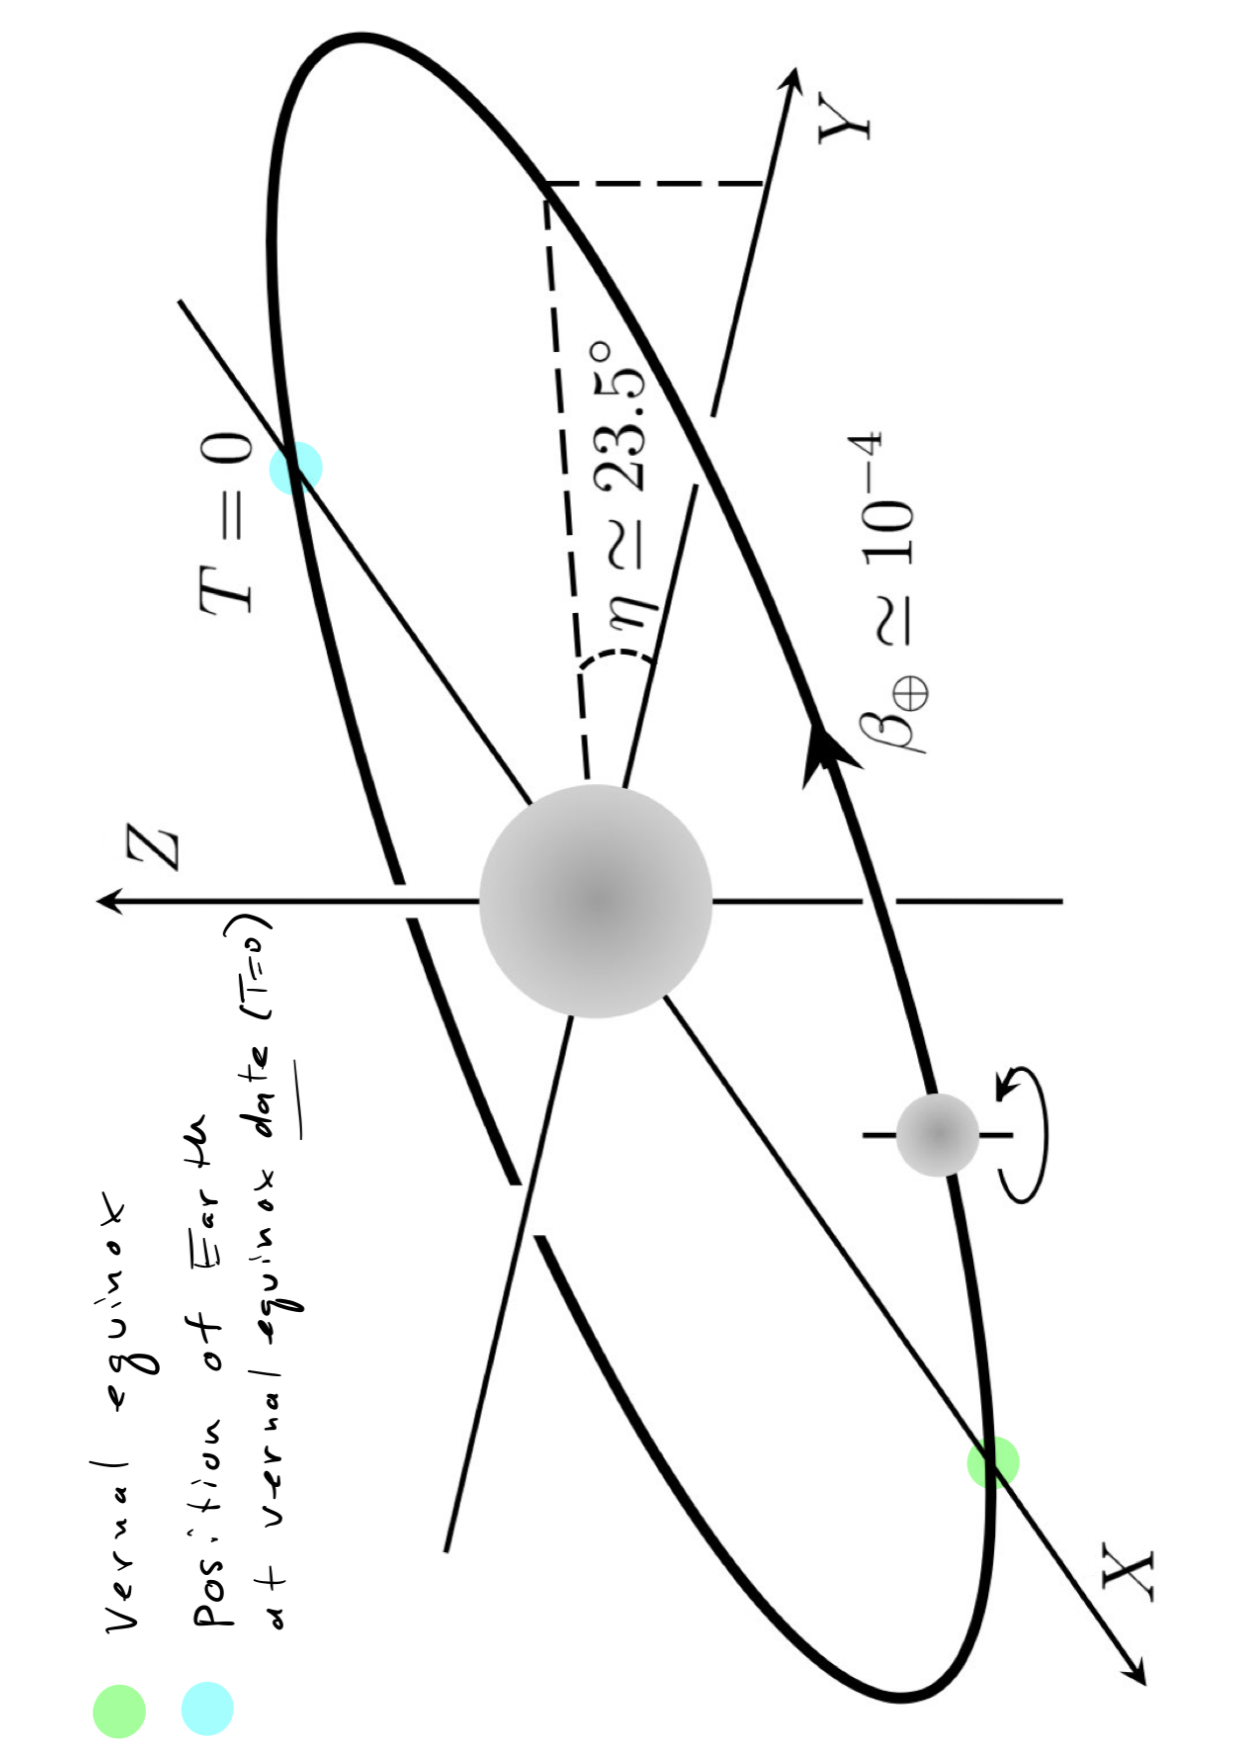
\includegraphics[scale=0.50,angle=-90]{figs/intro_theory/SCF_pic.pdf}
\caption{Edited illustration of the SCF (originally image from Ref.~\cite{kd16}). 
The Sun is the larger shaded disk in the center and
and the Earth the smaller disk revolving about the Sun. 
When looking down the Sun $Z$ axis, the Earth
is seen revolving counterclockwise in an approximately circular orbit 
and rotating counterclockwise about its rotation axis. 
The SCF axes are chosen such that $Z$ axis 
is parallel with the Earth's rotation axis. The orbit of the Earth
in this frame is inclined relative to the $X$-$Y$ plane
by $\eta \simeq 23.5^{\circ}$. 
The $X$-$Y$ plane is parallel to the
Earth's equatorial plane. The vernal equinox 
is the point where the $X$ axis intersects 
the Earth's orbit (green dot). On the date 
of the 2000 vernal equinox the Earth 
is positioned at the light-blue dot near $T=0$. 
At this latter dot, the $X$ axis intersects the Earth
and points from the Earth to the Sun.
At this moment, there is one position on the Earth's equator where an observer 
would see the Sun directly overhead (toward their local zenith)
at noon local time. The longitude of this location is given by $\lambda_0$
from Eq.~\eqref{angularshift}.}
\label{fig:scf}
\end{figure}
%
Next, the canonical frames used to describe the
laboratory apparatus frame and its connection
to the SCF are introduced.
%
%
\subsection{Standard laboratory frame}
%
%
The \textit{standard laboratory frame}
is a fixed frame on the surface of the Earth, and
hence rotates with respect to the SCF. 
The coordinates of this frame are 
defined as $x^j \equiv (x,y,z)$, where
the $x$ axis points toward local south, the $y$ axis toward
local east, and the $z$ axis toward the local zenith. 
%
It is convenient to identify the 
standard laboratory frame time coordinate $t$ 
with the local sidereal time $T_\oplus$.
The local sidereal time is defined to have 
an origin $T_\oplus = 0$ when the laboratory $y$ axis 
is parallel to the Sun $Y$ axis, $y||Y$. 

Under the approximation that the Earth moves in a circular
orbit around the Sun, the transformation from the 
SCF to the standard laboratory frame 
is given by a rotation $R^{jJ}$ such that 
%
\begin{equation}
x^j = R^{jJ}X^J,
\end{equation}
%
where the sum over the repeated index $J$ is implied.
To determine $R^{jJ}$, we imagine that the coordinates $x^j$ and
$X^J$ are initially parallel and with coincident origins. 
From the viewpoint of $X^J$,
the coordinates $x^j$ appear to be rotating.
So, first a rotation about the $Z$
axis by an angle $\omega_\oplus T_\oplus$ is performed:
%
\begin{equation}
R_{Z} = \begin{pmatrix} \cos\omega_\oplus T_\oplus 
& \sin\omega_\oplus T_\oplus & 0 \\ 
-\sin\omega_\oplus T_\oplus 
& \cos\omega_\oplus T_\oplus & 0 \\ 0 & 0 & 1 \end{pmatrix}.
\end{equation}
%
In looking down the $Z$ axis, the $x$ and $y$ axes will be rotating
counterclockwise in the $X$-$Y$ plane. 
This is consistent with the fact that
the Earth rotates counterclockwise about
its own axis when viewed from the northern hemisphere. 
Next, a second rotation is needed 
to make $\widehat{z}\cdot\widehat{Z} = \cos\chi$,
where $\chi$ is the colatitude of the 
standard laboratory\footnote{the hat notation indicates unit vectors}.
This is achieved by a counterclockwise 
rotation about the $Y$ axis by an angle $\chi$:
%
\begin{equation}
R_{Y} = \begin{pmatrix} \cos\chi & 0 & -\sin\chi \\ 
0 & 1 & 0 \\ \sin\chi & 0 & \cos\chi\end{pmatrix}.
\end{equation}
%
Thus, the net rotation is now $R^{jJ} = R_{Y}\cdot R_{Z}$ and given by
%
\begin{equation}
\label{RjJ}
R^{jJ} = \begin{pmatrix} \cos\chi\cos\omega_\oplus T_\oplus & \cos\chi\sin\omega_\oplus T_\oplus 
& -\sin\chi \\ -\sin\omega_\oplus T_\oplus & \cos\omega_\oplus T_\oplus & 0
\\ \sin\chi\cos\omega_\oplus T_\oplus & \sin\chi \sin\omega_\oplus T_\oplus & \cos\chi
\end{pmatrix}.
\end{equation}
%
Note this is Eq. (44) in Ref.~\cite{kd16}.
For more information on the 
standard laboratory frame, see Ref.~\cite{km02}. 
An illustration depicting the rotation~\eqref{RjJ} is 
given in Ref.~\cite{k2000}. 

Connecting other laboratory frames, 
such as the ATLAS detector frame, to the SCF can be achieved by 
applying additional rotations following $R^{jJ} = R_Y\cdot R_Z$ given in Eq.~\eqref{RjJ}.
%
%
\subsection{ATLAS detector frame}
%
We now describe additional rotations that must be performed to
connect the ATLAS frame to the SCF. 

Recall that the standard laboratory frame (positive) $y$ axis
points to local east.
At the ATLAS detector interaction point the collider ring
has its beamlines oriented at some angle $\psi$ north of east.
The following matrix rotates the $y$ axis to this direction:
%
\begin{equation}
\label{psirot}
\begin{pmatrix} \cos\psi & \sin\psi & 0 \\ 
-\sin\psi& \cos\psi& 0 \\ 0 & 0 & 1 \end{pmatrix}.
\end{equation}
%
Note that $y$ is now pointing along 
the ATLAS ``beamline 1" direction.
As is typically chosen, the beam-direction
axis is in the $\widehat{z}$ direction. A transformation
that swaps the $y$ and $z$ axes is 
%
\begin{equation}
\label{Rswap}
\begin{pmatrix} \pm 1 & 0 & 0
\\ 0 & 0 & 1 \\ 0 & \mp 1 & 0 
\end{pmatrix}.
\end{equation}
%
The upper (lower) signs orient $\widehat{z}$ antiparallel (parallel) 
to the prior $\widehat{y}$ direction. 
For either sign the final $\widehat{y}$ 
direction points toward the local zenith.
Applying Eqs.~\eqref{psirot},\eqref{Rswap} after
Eq.~\eqref{RjJ} results in the rotation used in studies involving the 
HERA/EIC colliders in \cite{klv17, ls18}. For ATLAS, 
one final transformation needed because the ATLAS detector 
is slightly inclined relative to the $\widehat{z}$
direction. Performing a rotation of $-\delta$ around the $\widehat{x}$
direction achieves 
this\footnote{Our conventions for rotations are that
a positive angle is associated with a counterclockwise rotation. Here
we have a clockwise rotation around the $x$ axis, hence the minus sign.}:
%
\begin{equation}
\begin{pmatrix} 1 & 0 & 0 \\ 0 & \cos(-\delta) & \sin(-\delta) \\ 
0 & -\sin(-\delta)& \cos(-\delta) \end{pmatrix}.
\end{equation}
%

In total, the net rotation converting 
the SCF coordinates to the ATLAS coordinates is found to be
%
\begin{align}
\label{Rnet}
R(T_\oplus) = \begin{pmatrix} 1 & 0 & 0
\\ 0 & \cos\delta & -\sin\delta \\ 0 & \sin\delta & \cos\delta
\end{pmatrix}&\begin{pmatrix} + 1 & 0 & 0
\\ 0 & 0 & 1 \\ 0 & - 1 & 0 
\end{pmatrix}
\begin{pmatrix} \cos\psi & \sin\psi & 0 \\ 
-\sin\psi& \cos\psi& 0 \\ 0 & 0 & 1 \end{pmatrix} \nonumber \\
&\times\begin{pmatrix} 
\cos\chi\cos\omega_\oplus T_\oplus & \cos\chi\sin\omega_\oplus T_\oplus 
& -\sin\chi \\ -\sin\omega_\oplus T_\oplus & \cos\omega_\oplus T_\oplus & 0
\\ \sin\chi\cos\omega_\oplus T_\oplus & \sin\chi \sin\omega_\oplus T_\oplus & \cos\chi
\end{pmatrix}.
\end{align}
%
The chosen sign in the $y\leftrightarrow z$ swap
matrix (Eq.~\eqref{Rswap}) identifies the 
beam $\widehat{z}$ direction with the ATLAS
``beam 2 direction"---see the ATLAS New Small Wheel TDR, Section 3.6.1, pg. 24.
The numerical values of the relevant angles are
%
\begin{align}
\label{angularvalues}
&\chi = 43.764290859^\circ, \\
&\psi = 168.7^\circ, \\
&\delta = |-\delta| = |-0.704^\circ| = + 0.704^\circ.
\end{align}
%
Note the minus sign in $\delta$ is taken into account in Eq.~\eqref{Rnet}.
For an expanded discussion of the SCF, standard
laboratory frame, and laboratory apparatus frame, see
Ref.~\cite{km09}.
%
%
\subsubsection{Explicit example}
\label{sec:phase_comp}
%
%
As a simple example, consider again our archetypal LIV effect:
${\cal L}_b = -b_\mu \bar \psi \gamma_5\gamma^\mu \psi$
from Eq.~\eqref{bterm}. Let us imagine we are working in the ATLAS detector frame.
Then $b_\mu = (b_0, b_j) $ has components decomposed 
in the coordinate basis describing this frame.
Noting Eq.~\eqref{Rnet}, we wish to express
$b_\mu$ in terms
of the fixed SCF frame coefficients, which we call
$b_{\text{SCF}}^\mu = (b^T, b^X, b^Y, b^Z)$.
Since the ATLAS detector and SCF differ by a coordinate 
transformation (Lorentz observer transformation), the 
coeffcient $b_\mu$ transforms like a usual four-vector:
%
\begin{align}
\label{blabSCF}
b^\mu = [R(T_\oplus)]^\mu_{\hphantom{\mu}\nu} b_{\text{SCF}}^{\nu},
\end{align}
%
where
$[R(T_\oplus)]^\mu_{\hphantom{\mu}\nu}$ is the four-dimensional
version of the spatial rotation matrix $R(T_\oplus)$ from Eq.~\eqref{Rnet}. 
The additional elements are $R^0_{\hphantom{0}0} = 1, 
R^0_{\hphantom{0}j} = R^j_{\hphantom{j}0} = 0$. 
As a simplifying limit, and 
without loss of generality, consider $\delta \rightarrow 0$. 
%
\begin{figure}[ht]
\centering
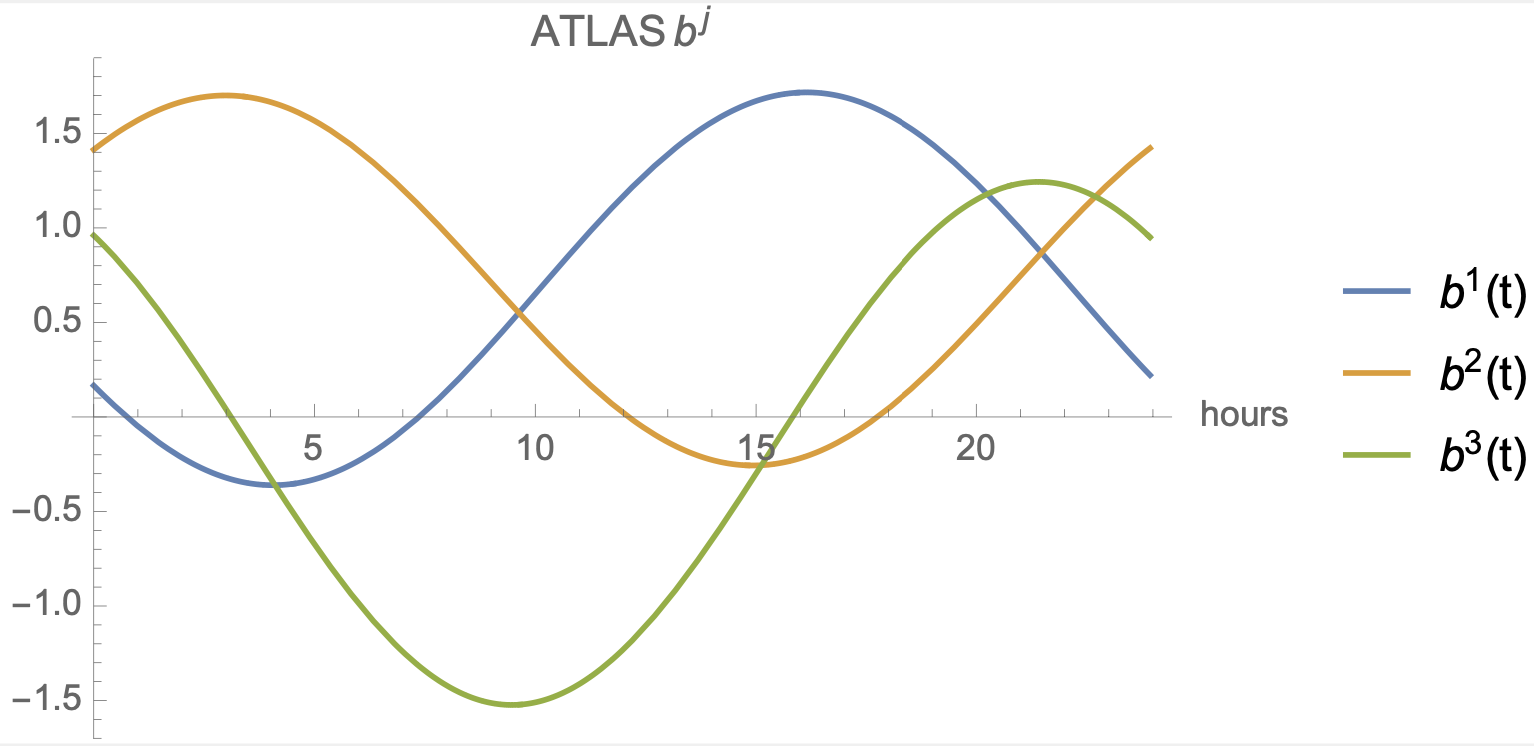
\includegraphics[scale=0.40]{figs/intro_theory/ATLASbj.png}
\caption{Components $b^j$ from Eq.~\eqref{ATLAScomps} 
plotted over a sidereal day for $b_{\text SCF}^J \equiv  1$. 
The (small) effects of setting $\delta = |-0.704^\circ|$ are also included.}
\label{fig:ATLASbj}
\end{figure}
%
It is then found that
%
\begin{align}
\label{ATLAScomps}
b^0 = \; & b^T \\
b^1 = \; & -b^Z\sin\chi\cos\psi + \cos(\omega_\oplus T_\oplus)(b^X\cos\chi\cos\psi + b^Y\sin\psi) \nonumber \\
      & + \sin(\omega_\oplus T_\oplus)(b^Y\cos\chi\cos\psi - b^X\sin \psi) \\
b^2 = \; & b^Z\cos\chi + b_X\cos(\omega_\oplus T_\oplus)\sin\chi + b_Y\sin(\omega_\oplus T_\oplus)\sin\chi  \\
b^3 = \; & -b^Z\sin\chi\sin\psi + \cos(\omega_\oplus T_\oplus)(b^X\cos\chi\sin\psi - b^Y\cos\psi) \nonumber \\
      \; & + \sin(\omega_\oplus T_\oplus)(b^Y\cos\chi\sin\psi + b^X\cos\psi)
%
%\begin{pmatrix} b^0 \\ b^1 \\ b^2 \\ b^3 
%\end{pmatrix} 
%= 
%\begin{pmatrix} b^T \\ -b^Z\sin\chi\cos\psi + \cos(\omega_\oplus T_\oplus)(b^X\cos\chi\cos\psi + b^Y\sin\psi)
%+ \sin(\omega_\oplus T_\oplus)(b^Y\cos\chi\cos\psi - b^X\sin \psi) \\
%b^Z\cos\chi + b_X\cos(\omega_\oplus T_\oplus)\sin\chi + b_Y\sin(\omega_\oplus T_\oplus)\sin\chi \\
%-b^Z\sin\chi\sin\psi + \cos(\omega_\oplus T_\oplus)(b^X\cos\chi\sin\psi - b^Y\cos\psi)
%+ \sin(\omega_\oplus T_\oplus)(b^Y\cos\chi\sin\psi + b^X\cos\psi)
%\end{pmatrix}.
\end{align}
%
We observe that the time dependence has been made explicit through
the functions $\cos(\omega_\oplus T_\oplus), \sin(\omega_\oplus T_\oplus)$. 
See Fig.~\ref{fig:ATLASbj}
for the resulting time dependence of the ATLAS 
components. Note that all
components have a distinct shape and that even
in the absence of time-dependent effects
there is a unique dependence on the laboratory location
through the angles $\chi, \psi$. 

For more complicated LIV backgrounds, like $c$- and $d$-type coefficients
introduced in Sec.~\ref{ssec:canddtype}, additional applications of the net rotation
matrix must be performed. For example,
%
\begin{equation}
\label{cuexample}
(c_{u_i})^{\mu\nu} = \left[R(T_\oplus)\right]^\mu_{\hphantom{\mu}\alpha}
\left[R(T_\oplus)\right]^\nu_{\hphantom{\nu}\beta}(c_{u_i})_{\text{SCF}}^{\alpha\beta},
\end{equation}
where the parentheses () have been introduced for clarity.
%
%
\subsubsection{Another explicit example}
\label{sec:phase_comp1}
%
%
We now revisit the cross section $d\sigma/dQ^2$ from Eq.~\eqref{DYsigmadQ2}.
It involves combinations of the coefficients
described in Eq.~\eqref{eq:quarkcoeffs}. Evaluation of $d\sigma/dQ^2$ in the
ATLAS detector frame reveals that the only time-dependent
coefficients that appear are $c_f^{33}, d_f^{33}$. We must re-express
these coefficients in terms of the SCF 
coefficients using, e.g., Eq.~\eqref{cuexample}. 
We find
%
\begin{align}
\label{c33}
c_{f}^{33} =&
\frac{1}{2}(c_{f}^{XX} + c_{f}^{YY})\left(\cos^2\chi\sin^2\psi + \cos^2\psi\right) +  c_{f}^{ZZ}\sin^2\chi\sin^2\psi
\nonumber\\
& - 2c_{f}^{XZ}\sin\chi\sin\psi
\left[\cos\chi\sin\psi\cos(\omega_{\oplus}T_{\oplus} )
+ \cos\psi\sin(\omega_{\oplus}T_{\oplus})\right]
\nonumber\\
& - 2c_{f}^{YZ}\sin\chi\sin\psi
\left[\cos\chi\sin\psi\sin(\omega_{\oplus}T_{\oplus})
- \cos\psi\cos(\omega_{\oplus}T_{\oplus})\right] \nonumber\\
& + c_{f}^{XY}\left[(\cos^2\chi\sin^2\psi - \cos^2\psi)\sin(2\omega_\oplus T_\oplus) - \cos\chi\sin(2\psi)\cos(2\Omega_\oplus T_\oplus)    \right] \nonumber \\
& +\frac{1}{2}(c_{f}^{XX} - c_{f}^{YY})\left[(\cos^2\chi\sin^2\psi - \cos^2\psi)\cos(2\omega_\oplus T_\oplus) \right. \nonumber\\
& \left.+ \cos\chi\sin(2\psi)\sin(2\omega_\oplus T_\oplus)\right],
\end{align}
%
and similarly for $d_f^{33}$. 
We see that the coefficients with SCF superscript 
indices $XX+YY$ and $ZZ$ are only associated to time-independent effects. 
Those with indices $XZ, YZ, XY, XX-YY$ introduce 
sidereal time-dependent effects and are of primary interest.
Inserting 
Eq.~\eqref{c33} into the laboratory-frame
expression of Eq.~\eqref{DYsigmadQ2} and
noting the constraint
%
\begin{equation}
c_{u_i}^{\mu\nu} - c_{d_i}^{\mu\nu} = d_{d_i}^{\mu\nu} - d_{u_i}^{\mu\nu},
\end{equation}
%
results in the observable of interest for our analysis.
%
%
\subsection{Initial conditions and shifts}
\label{sec:timeshift}
%
%
The previous sections focused on the spatial transformation from the 
SCF to the ATLAS detector frame and the implications for observables. 
In this section, we describe an important temporal transformation
that must be accounted for.

We begin by asking:
%
\begin{itemize}
\centering
\item[] \emph{Where on the equator at the vernal equinox 2000 ($T=0$)
is the Sun directly overhead (at noon local time)?}
\end{itemize}
%
At this location, the standard laboratory frame $z$ axis
is oriented such that 
$\widehat{z} \parallel \widehat{X}$, $\widehat{y} \parallel \widehat{Y}$, 
and $T = T_\oplus = 0$, assuming the origin of 
$T_\oplus$ is chosen to occur on the equinox date. This location
is found by noting there are 
$(4 + \frac{25}{60} \simeq 4.417)$ local hours that 
must elapse for the Sun to be approximately overhead at noon in the UTC 
timezone at longitude 0$^{\circ}$ (recall that the equinox
occurs at 7:35 am UTC). Therefore, the Sun
is overhead on the equator at a longitude \emph{advanced} by 
\begin{align}
\label{angularshift}
\lambda_0 &= 4.417\;\text{hr}\cdot\frac{2\pi}{24 \text{hr}}
\cdot\frac{180}{\pi} \nonumber\\
&= 66.25^{\circ},
\end{align}
which is in the Indian Ocean west of the Maldives, matching the claim 
in Ref.~\cite{kd16}. 
Note it is only at $\lambda_0$
that a (hypothetical) laboratory with $T = T_\oplus$ has its local zenith
pointing toward the Sun.

For a laboratory positioned at any other longitude, 
$\widehat{y} \parallel \widehat{Y}$ at an earlier
or later time than the equinox.  
Given the direction of Earth's rotation, 
for $\lambda < \lambda_0$, 
$T - T_\oplus > 0$, and for $\lambda > \lambda_0$, 
$T - T_\oplus < 0$. 
The time it takes for such laboratory to advance 
depends on a linear longitudinal shift,
and the time for $\widehat{y}$ to 
continually realign with $\widehat{Y}$ is a sidereal 
day with period 23 hr 56 min 4.091 s $\simeq$ 23.934 hr. 
This latter dependence on the sidereal day, 
as opposed to a 24-hour solar
day, is because the Earth is slightly changing
its angular position relative to the Sun
by an amount quantified by the sidereal day.
We find 
\begin{align}
\label{relation}
T - T_\oplus = \frac{\lambda_0 - \lambda}{360^{\circ}}\cdot 
(23.9344697\bar{2}\;\text{hr}),
\end{align}
which is Eq. (43) in Ref.~\cite{kd16} reported with higher precision. 
Note that this result is independent of the latitude of the laboratory. 
Also note that $T - T_\oplus$ can more generally depend
on a integer number $n$ of 
sidereal days, such that an 
additional shift $\frac{2\pi}{\omega_{\oplus}}n$
needs to be included on the right-hand side 
of Eq.~\eqref{relation} if the origin $T_\oplus = 0$ 
\textit{isn't} chosen on the 2000 vernal equinox date. 
%
As a relevant example, for ATLAS 
\begin{equation}
\lambda = 6.055279086^\circ,
\end{equation}
giving
\begin{align}
\label{TshiftATLAS}
T - T_\oplus\bigg|_{\text{ATLAS}} = 4.002\;\text{hr}.
\end{align}
Note that $2\times 10^{-3}\;\text{hr} = 7.28725\;\text{s}$. 
Thus, rounding to the nearest second, for the ATLAS 
experiment $\widehat{y}\parallel \widehat{Y}$ 
on March 20th, 2000 at 11:35:24 UTC.
It is this date and time 
that we identify with $T_\oplus\big|_{\text{ATLAS}} = 0$.
All data timestamps are assigned a 
unique $T_\oplus$ which is measured relative to this initial condition.
%
%\subsection{Example: $T_{\text Unix}$ comparison}

Since we have chosen to initialize our laboratory clock
with the local sidereal time, $t = T_\oplus$, 
every laboratory measurement comes with a time stamp $T_\oplus$.
However, suppose that events are instead known with 
respect to a different time origin, for instance
``Unix time", where $T_{\text{Unix}} = 0$ is defined as January 
1st, 0:00:00 UTC, 1970. To convert from Unix time to local time,
we must subtract off the difference
\begin{equation}
\label{Tshift}
(T_\oplus = 0) - (T_{\text{Unix} = 0}) = 953552124\;\text s
\end{equation}
from each event to compute how much time has elapsed since $T_\oplus = 0$. 
In Tab.~\ref{tab:datestimes} we 
compare the various dates and times discussed so far, as well as the sidereal
and solar phases with reference to $T_\oplus$ for ATLAS. 
%
\begin{table}
\centering 
\small
\begin{tabular}{c c c c c c c c} % centered columns (4 columns)
\hline\hline
event & calendar date & $T_{\text{Unix}}$
& $T$ & $T_\oplus$ & $\oplus\angle$ & $\odot\angle$ \\
%$\left(\frac{\mathcal{O}_{\rm SME}}{\mathcal{O}_{\rm SM}}-1\right)$  \\
\hline
1&$|$ 01/01/1970 00:00:00$|$& 0 $\qquad\qquad\hspace{.5mm}|$& -953537717
$|$& -953552124 $|$& 0.371415 $|$&  0.517083 \\
%
2&$|$ 01/01/2000 12:00:00$|$& 946728000 $\hspace{.5mm}|$& -6809717 $\quad|$& -6824124 $\quad|$& 0.35914 $\hspace{1.75mm}|$& 0.0170833\\
%
3&$|$ 20/03/2000 07:35:17$|$& 953537717 $\hspace{.5mm}|$& 0 $\qquad\qquad\hspace{1.0mm}|$& -14407 $\qquad|$& 0.857198 $|$& 0.833252\\
%
4&$|$ 20/03/2000 11:35:24$|$& 953552124 $\hspace{.5mm}|$& 14407 $\qquad\hspace{1mm}|$& 0 $\qquad\qquad\hspace{1mm}|$& 0 $\qquad\quad\hspace{1mm}|$& 0\\
%
5&$|$ 25/01/2021 18:49:42$|$& 1611600582$|$& 658062865  $\hspace{1mm}|$& 658048458 $\hspace{1mm}|$& 0.590071 $|$& 0.301597 \\
%
6&$|$ 25/03/2021 18:49:42$|$& 1616698182$|$& 663160465 $\hspace{1mm}|$& 663146058 $\hspace{1mm}|$& 0.117588 $|$& 0.301597 \\
\hline\hline 
\end{tabular}
\caption{Times other than the calendar date (GMT) are given in seconds. Sidereal ($\oplus\angle$) and solar ($\odot\angle$) phases are calculated
with respect to $T_\oplus$ for ATLAS.}
\label{tab:datestimes}
\end{table}
%
Alternatively, the bin for a given event $T_\oplus$ may be calculated from
\begin{align}
\text{bin \#} =  
\text{mod}\left[\frac{T_\oplus - \text{mod}[T_\oplus,\frac{2\pi}{n\omega_\oplus}]}
{\frac{2\pi}{n\omega_\oplus}},n\right] + 1, 
\label{eq:sid_phase_bin}
\end{align}
where $n$ is the number of bins (intervals) the sidereal day has been split into. For example, 
for $n=1$ the length of the interval is the sidereal day, which
is 23.94 hr. For $n=2$, there are two intervals of duration 23.94/2 = 11.97 hr, 
and so on. 



\subsection{Minimal SME coefficients probed in this analysis}
\label{subsec:WC}

As shown in Sec.~\ref{sec:phase_comp}, for a given flavor $f$
there are four coefficient types $XZ, YZ, XY, XX-YY$ that induce
sidereal time dependence in the Drell-Yan dilepton distribution 
$d\sigma/dQ^2$. In the basis of $c$- and 
$d$-coefficients (Eq.~\eqref{eq:quarkcoeffs}) there are
three independent coefficient types per generation. This gives
$3\times 4 = 12$ coefficients for $(u,d)$ quarks and 12 more 
for $(s,c)$ quarks. Note that we are not sensitive to 
the third generation $(b,t)$. Together this gives 24 SME coefficients.
%We plan to probe 24 Wilson coefficients which 
%have the time-dependent behaviour:\footnote{For an example of 
%how the numerical prefactors in the equations that follow 
%depend on the ATLAS laboratory coordinates and sidereal quantities 
%see, e.g., Eq. (4.19) of Ref.~\cite{Kostelecky:2016pyx}, where 
%$\Omega_\oplus = \omega_\oplus = 
%2\pi/(23\;\text{hr}\;56\;\text{min}\;4.091\;\text{s})$
%is the Earth's sidereal frequency 
%and $T_\oplus$ is the local sidereal time.}
%
For the first generation, the functional dependence attached to 
each coefficient is given by
%
\begin{eqnarray}
  d_u^{XZ} &:& 6.28069 \cos(\omega_\oplus T_\oplus)-41.0569 \sin(\omega_\oplus T_\oplus) 
               = 41.5345 \cos (\omega_\oplus T_\oplus+ 1.419) \label{eq:duXZ}\\
  d_u^{YZ} &:& 41.0569 \cos(\omega_\oplus T_\oplus)+6.28069 \sin(\omega_\oplus T_\oplus)   
               = 41.5345 \cos (\omega_\oplus T_\oplus+ 0.151798) \label{eq:duYZnum}       \\
  d_u^{XX-YY} &:& 77.6067 \cos(2\omega_\oplus T_\oplus )+24.3128 \sin(2\omega_\oplus T_\oplus ) 
               = 81.326 \cos (2 \omega_\oplus T_\oplus+ 0.303597)  \\
  d_u^{XY} &:& -48.6256 \cos(2\omega_\oplus T_\oplus )+155.213 \sin(2\omega_\oplus T_\oplus )
               = 162.652 \cos (2 \omega_\oplus T_\oplus+ 1.87439)  \\
  c_u^{XZ} &:& 8.084 \cos(\omega_\oplus T_\oplus)-52.8451 \sin(\omega_\oplus T_\oplus)            
                 = 53.4599 \cos (\omega_\oplus T_\oplus+ 1.419) \\
  c_u^{YZ} &:& 52.8451 \cos(\omega_\oplus T_\oplus)+8.084 \sin(\omega_\oplus T_\oplus)            
               = 53.4599 \cos (\omega_\oplus T_\oplus+ 0.151798)      \\
  c_u^{XX-YY} &:& 99.8891 \cos(2\omega_\oplus T_\oplus )+31.2935 \sin(2 \omega_\oplus T_\oplus)  
                 = 104.676 \cos (2 \omega_\oplus T_\oplus+ 0.303597)  \\
  c_u^{XY} &:& -62.5869 \cos(2\omega_\oplus T_\oplus )+199.778 \sin(2\omega_\oplus T_\oplus )      
                 = 209.352 \cos (2 \omega_\oplus T_\oplus+ 1.87439)  \\
  c_d^{XZ} &:& 0.181551 \cos(\omega_\oplus T_\oplus)-1.1868 \sin(\omega_\oplus T_\oplus)           
                 = 1.20061 \cos (2 \omega_\oplus T_\oplus+ 1.87439)  \\
  c_d^{YZ} &:& 1.1868 \cos(\omega_\oplus T_\oplus)+0.181551 \sin(\omega_\oplus T_\oplus)           
                   = 1.20061 \cos (\omega_\oplus T_\oplus+ 1.419) \\
  c_d^{XX-YY} &:& 2.24331 \cos(2\omega_\oplus T_\oplus )+0.702788 \sin(2 \omega_\oplus T_\oplus) 
                   = 2.35082 \cos (2 \omega_\oplus T_\oplus+ 0.303597)  \\
  c_d^{XY} &:& -1.40558 \cos(2\omega_\oplus T_\oplus )+4.48662 \sin(2 \omega_\oplus T_\oplus) 
                   = 4.70164 \cos (2 \omega_\oplus T_\oplus+ 1.87439)  \\
  \label{eq:cdXY}   
\end{eqnarray}
%
and similarly for $(u,d)\leftrightarrow(s,c)$. 
%Note these coefficients first appear
%in Eq.~\eqref{eq:quarkcoeffs} and control the Lorentz-violating corrections to 
%the dilepton distribution as described in Eq.~\eqref{sigmaprime}. 
Figure~\ref{fig:SME_effects} shows the signature of these
coefficients as a function of sidereal phase $\omega_\oplus T_\oplus$. Note that each
coefficient type is strictly associated with either first or second
harmonics of the sidereal phase $\omega_\oplus T_\oplus$. 
%
\begin{figure}[ht]
	\centering
	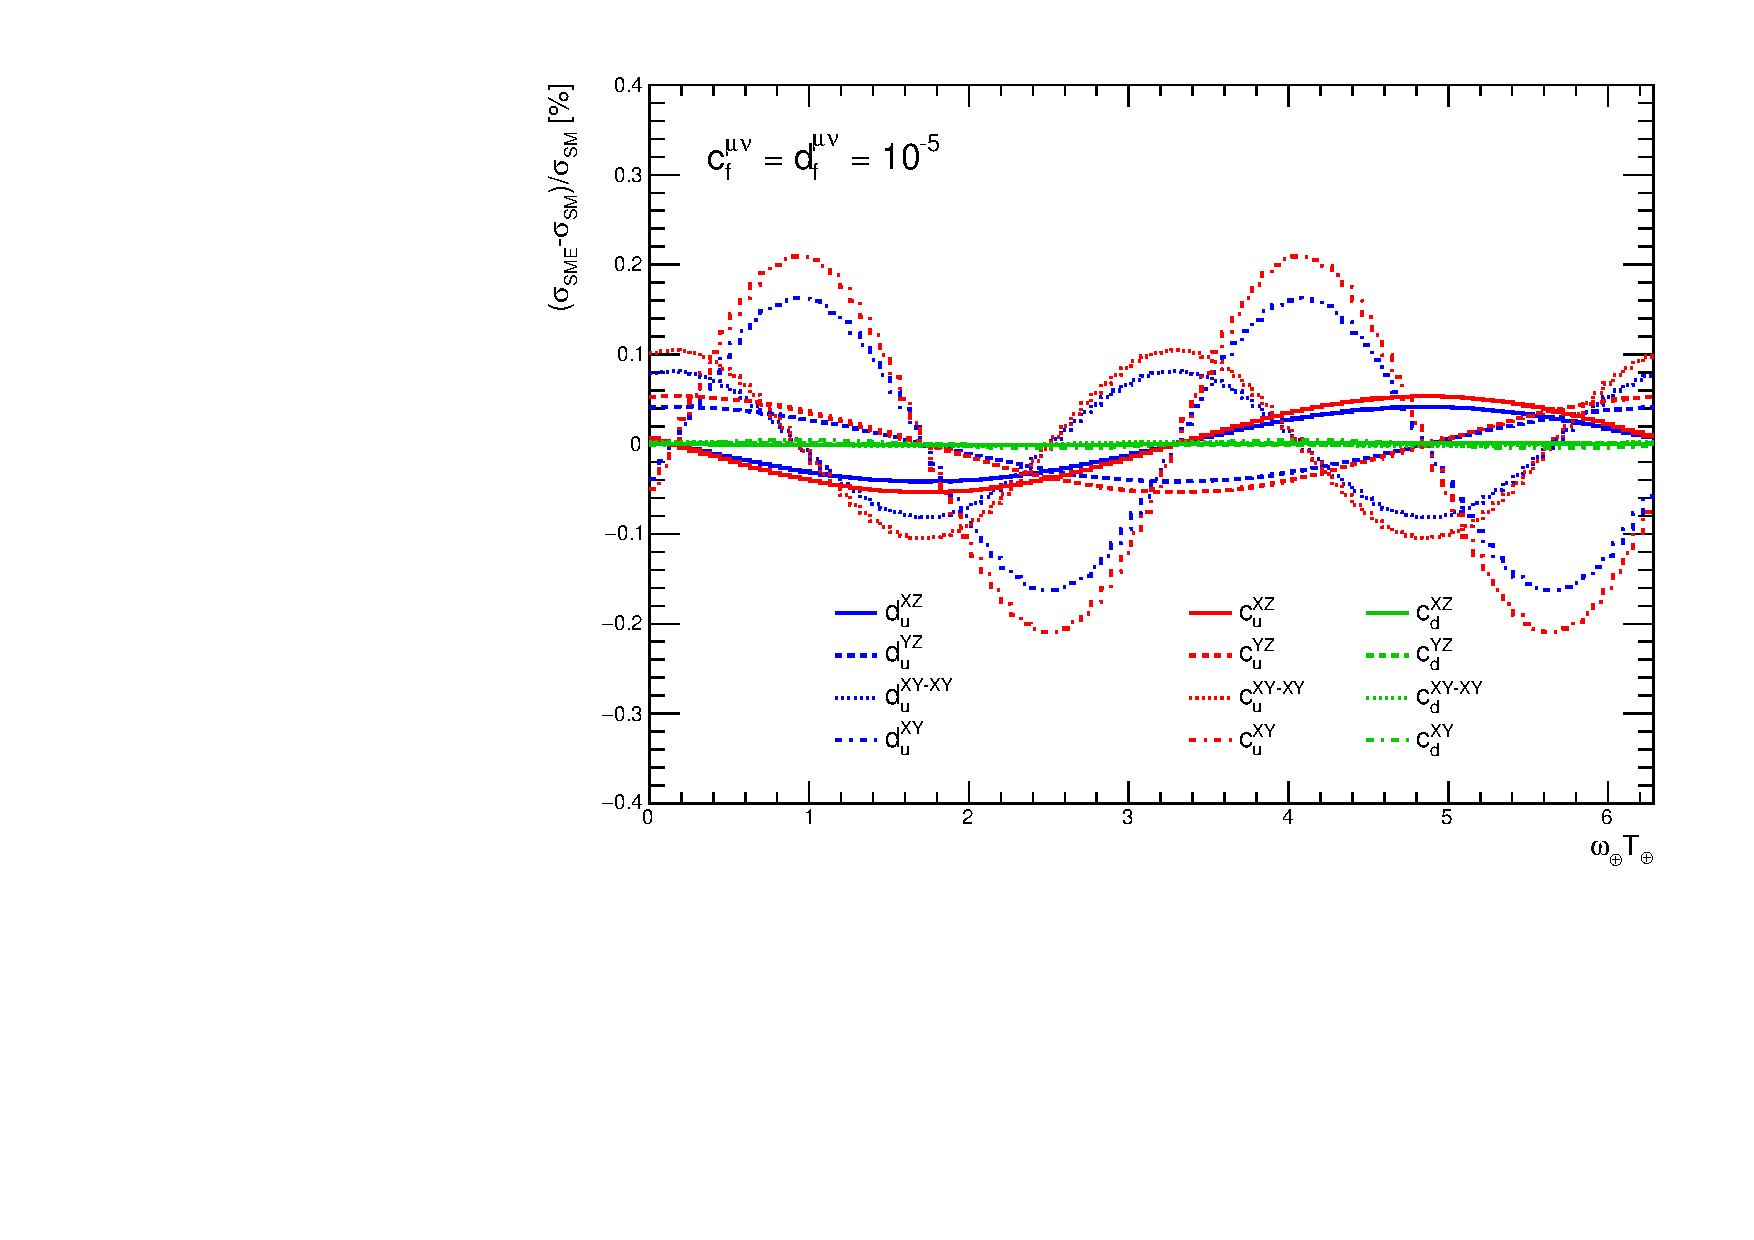
\includegraphics[scale=0.75]{figs/SMEeffects.pdf}
	\caption{Functional forms of the time dependence associated with 
    each SME coefficient, as expressed in 
    Eqs.~\ref{eq:duXZ}-\ref{eq:cdXY}.}
	\label{fig:SME_effects}
\end{figure}
%
%
\subsection{Nonminimal quark-sector effects}
%
%
Thus far we have focused on the minimal SME in the quark sector.
From an effective field theory viewpoint, nonrenormalizable operators 
of mass dimension $d>4$ parametrize the effects of new physics 
suppressed by the associated characteristic energy scale. The more
energetic a given process the more relevant nonrenormalizable operators
become. For example, a $d=5$ operator has a SME coefficient
with dimension GeV$^{-1}$. The dominant (tree-level) insertions of
this operator introduces an expansion parameter $\delta = (E/\Lambda)$,
where $E$ is the process scale (e.g. the energy
of the initial-state partons in the Drell-Yan procees), 
and $\Lambda$ the scale of new physics (e.g the Planck scale). 
The larger $E$ is, the more relevant the expansion parameter. A $d=6$
operator would include a leading-order correction controlled
by $\delta^2$. Though clearly suppressed relative to the
$d=5$ operator, since $\Lambda$ is fixed the influence of the $d=6$
operator grows more rapidly. Nonrenormalizable operators
are extensively studied in Lorentz-invariant new-physics
searches at the LHC because they generically
parametrize new physics too heavy to be 
produced on-shell by the colliding beamlines. 

Nonrenormalizable effects from the nonminimal SME 
have also been investigated in 
Drell-Yan dilepton production~\cite{Kostelecky:2019fse}. 
The $d=5$ Lagrange density was considered:
%
\begin{equation}
{\cal L}_{a^{(5)}} = -\frac{1}{2}\sum_f a_f^{(5)\mu\alpha\beta}
\bar\psi_f \gamma_\mu iD_{(\alpha}iD_{\beta)}\psi_f + \text{h.c.},
\end{equation}
where the parenthesis surrounding $\alpha, \beta$ denotes index symmetrization
and h.c. is shorthand for Hermitian conjugation. 
%
\begin{table}[t]
\centering
\begin{tabular}{|c|c|c|}\hline
& {\textbf{HERA}} & {\textbf{LHC}} \\ \hline
 $|a^{(5)TXX}_{\text{S}u}- a^{(5)TYY}_{\text{S}u} |$& $4.3\times 10^{-7}$ & $1.5\times 10^{-8}$ \\
 $|a^{(5)TXY}_{\text{S}u}|$& $6.5\times 10^{-7}$ & $2.7\times 10^{-9}$ \\
 $|a^{(5)TXZ}_{\text{S}u}|$ & $1.1\times 10^{-6}$ & $7.2\times 10^{-9}$ \\
 $|a^{(5)TYZ}_{\text{S}u} |$&  $7.4\times 10^{-7}$ & $7.0\times 10^{-9}$ \\
\hline
\end{tabular}
\caption{Comparison of HERA and LHC sensitivity to $a^{(5)}$-type coefficients.
The limits from HERA come from a recent ZEUS analysis~\cite{ZEUS:2022msi} and coincide with the
positive upper limit report in units of GeV$^{-1}$. 
The quoted values for LHC come from simulations assuming uncorrelated
systematic uncertainties. Table adapted from Refs.~\cite{Kostelecky:2019fse},\cite{ZEUS:2022msi}.
\label{tablea5}}
\end{table}
%
We will refer to the SME coefficients that 
appear as the $a^{(5)}$-type coefficients. From Table~\ref{tablea5} 
it is observed that the LHC could expect up to two orders 
of magnitude more sensitivity to these coefficients than what was obtained
by the ZEUS Collaboration~\cite{ZEUS:2022msi}. This increased sensitivity
has its origin in the increased collision energy of the LHC relative to HERA.

The predictions of Table~\ref{tablea5} are limited to photon exchange. When
electroweak bosons are exchanged, the $a^{(5)}$-type coefficients cannot be treated in isolation.
The reasons are exactly the same as for why the $c$-type coefficients
can not be treated independently of the $d$-type coefficients when
a $W^\pm$ or $Z$ is exchanged, as discussed in Sec.~\ref{ssec:LIVDY}. 
Analogous to the $d$-type coefficients, the other set of coefficients
relevant for the nonminimal effects probed here are called the $b^{(5)}$-type 
coefficients. 

Predictions for Drell-Yan on the $Z$ pole and including the
$b^{(5)}$-type coefficients are currently being calculated by
the theory STA members~\cite{LS24}. Because the $a^{(5)}$-
and $b^{(5)}$-type coefficients are analogous in structure to the
$c$- and $d$-type coefficients, we expect a similar enhancement
of nonminimal LIV signatures on the $Z$ pole. Therefore, it is reasonable
to expect a greater relative sensitivity to these coefficients
than estimated in Table~\ref{tablea5}. 

Since the $a^{(5)}$- and $b^{(5)}$-type coefficients have an odd number
of Lorentz indices, they also produce striking CPT-violating effects.
For example, in deep inelastic scattering, when summing
the antiquark contributions these coefficients appear with opposite
signs to the quark contributions. Thus, for the sea quarks in the proton
the effect cancels out. The ZEUS analysis was therefore only sensitive
to the $u$ and $d$ quark $a^{(5)}$ coefficients. In contrast,
the leading Drell-Yan diagram involves $q\bar q$ fusion. The appearance
of particle and antiparticle in this diagram does not
produce the same cancellation effect as in deep inelastic scattering. 
Therefore, the Drell-Yan process can probe the CPT properties
of quarks. Our analysis will be the first probe of the CPT 
properties of sea quarks.



